% Provenance (never printed): see sources/outline_sources.md (Year 2: taphonomy; index fossils;
% facies and fossils as environment markers; reconstructing a palaeoenvironment from a map and a
% section). Taphonomy after Loron (2024); live, dead and fossil assemblages after Tyler and
% Kowalewski (2025); Lagerstaetten after Gaines and others (2024), Mussini and Butterfield
% (2025), Vannier and others (2018), Gerschermann and others (2021) and Rauhut and others
% (2018); zone durations after Al-Suwaidi and others (2022); ichnofacies after Buatois and others
% (2020) and Paz and others (2023); stenohaline groups after McGairy and others (2021) and Saleh
% and others (2022). The Varden column from figdata/shared/region.py; porosities and rates from
% figdata/bachelor-2/palaeoenv.py; exercise and problem values in the Book 4 scratch calculator
% calc/ch20.py. The fossil content given to the Varden units is invented, like the region.
\chapter{الحفريات والبيئات القديمة}\label{ch:b2:palaeoenvironments}

على لوح من الحجر الرملي الرمادي ثلاثة أدلّة: الأثر الذي حرثه ثلاثيّ فصوص في الطين،
والتموّجات التي خلّفها تيّار، وجحر حفرته دودة ثم هجرته. ليس أيّ منها حيوانًا كاملًا،
ومع ذلك تقول مجتمعةً إن هذا السفح كان يومًا قاع بحر، ضحلًا بما يكفي لتحرّكه الأمواج،
ومالحًا بما يكفي لتعيش فيه ثلاثيات الفصوص. الحفريات بقايا الحياة الماضية وآثارها،
ويقرؤها الجيولوجيون مرّتين: ساعاتٍ تؤرّخ الصخر، وشهودًا على المكان الذي تكوّن فيه.
يتتبّع هذا الفصل كائنًا حيًّا من موته إلى درج جامع الحفريات، ويفتح الرواسب النادرة
التي تبقى فيها حتى الأجسام الرخوة، ثم يقرأ بيئة بحر زائل، بالأرقام، في غطاء تلال
فاردن.
% ledger: usgs:fossil-record-bulk, loron24:taphonomy

\begin{recall}
\textbf{من مجلّدات المدرسة}: الحفرية، والقالب الخارجي والقالب الداخلي، \omterm{def:b2:palaeoenvironments:fossil-kinds}{والحفرية الأثرية}؛ وكيف
يحوّل الدفن والمعادن صدفةً إلى حجر؛ وتتابع الحفريات عبر الزمن. \textbf{من مجلد السنة الأولى}:
السحنات الرسوبية والبيئات الترسيبية، والعكرات، والشعاب والأويدات؛ والحيّزات الأحيائية، والحفريات
الدليلية ومعطيات الظهور الأول؛ والانضغاط، وفكّ الانضغاط، وقانون أثي والسماكة الصلبة
لطبقة؛ والملاط؛ والاستيعاب. \textbf{من الفصول السابقة}: التجاوزات والانحسارات البحرية،
ومستوى البحر الطويل الأمد \omterm{def:b2:phanerozoic-earth:oae}{وأحداث نقص الأكسجين المحيطي} (\cref{ch:b2:phanerozoic-earth}). أمّا كيف
تتطوّر الأنواع، وكيف تُصنَّف الحيوانات والنباتات، فمن شأن كتب الأحياء.
\end{recall}

\section{من الموت إلى الحفرية}\label{sec:b2:palaeoenvironments:taphonomy}

معظم الكائنات الحيّة لا تترك شيئًا وراءها. فالبكتيريا والكانسات تستهلك الأجزاء الرخوة في
أيام أو سنوات، والتيّارات تكسر الأجزاء الصلبة وتبعثرها، وأحماض التربة ومياه المسام
تذيب ما يبقى. الحفرية هي ما ينجو من هذا كلّه، ثم ينجو مرّة أخرى من دفن الصخر الذي
يحويها ومن تسخينه ورفعه.

\begin{definition}[علم التحفّر؛ قابلية الحفظ]\label{def:b2:palaeoenvironments:taphonomy}
\emph{علم التحفّر}\index{علم التحفّر} (التافونومي) دراسة ما يحدث لبقايا كائن حيّ
منذ موته حتى اكتشافه حفريةً: التحلّل، والكنس، والنقل، والدفن، والتغيّرات
الكيميائية في أثناء التحوّل الرسوبي. و\emph{قابلية الحفظ}\index{قابلية الحفظ}
لكائن حيّ، أو لجزء منه، هي احتمال أن يجتاز هذه المراحل
ويبقى في الصخر.
\end{definition}
% ledger: loron24:taphonomy

كلّ مرحلة تزيل شيئًا، أو تضيف شيئًا، أو تغيّر شيئًا. فالتحلّل والكنس يزيلان
الأنسجة الرخوة؛ والمعادن الآتية من مياه المسام تملأ مسامّ العظم أو تحلّ محلّ أراغونيت
الصدفة، فتضيف مادّة لم يملكها الحيوان قطّ؛ والتسخين يبدّل الجزيئات العضوية الباقية.
ويصنّف لورون هذه التغيّرات اللاحقة للموت كلّها في ثلاثة أنواع، الكسب والفقد والتبدّل،
ويكتبها معادلةً واحدة لتغيّر أيّ سمة قابلة للقياس بين الكائن الحيّ
وحفريته. ويتتبّع الشكل أدناه المراحل وما تنتزعه كلّ منها.
% ledger: loron24:taphonomy

\begin{omfigure}
\centering
\begin{tikzpicture}[font=\scriptsize, x=1cm, y=1cm,
  stage/.style={draw=black!60, fill=omSea!12, rounded corners=2pt, align=center,
    text width=2.05cm, minimum height=1.25cm, inner sep=2pt},
  loss/.style={align=center, text width=2.05cm, text=omThm!80!black}]
\node[stage] (a) at (0,0) {\textbf{الموت}\\مجتمع\\حيّ};
\node[stage] (b) at (2.75,0) {\textbf{التحلّل}\\\textbf{والكنس}\\على القاع};
\node[stage] (c) at (5.5,0) {\textbf{النقل}\\التيّارات تفرز\\وتكسر};
\node[stage] (d) at (8.25,0) {\textbf{الدفن}\\تحت الطبقة\\النشطة};
\node[stage] (e) at (11,0) {\textbf{التحوّل الرسوبي}\\\foreignlanguage{arabic}{الانضغاط،}\\الإحلال};
\node[stage] (f) at (13.75,0) {\textbf{الاستخراج}\\ثم\\الجمع};
\foreach \u/\v in {a/b, b/c, c/d, d/e, e/f} {\draw[-{Stealth[length=2mm]}, black!70] (\u) -- (\v);}
\node[loss, anchor=north] at (2.75,-0.8) {\foreignlanguage{arabic}{تضيع الأنسجة الرخوة؛}\\وتتفكّك الهياكل};
\node[loss, anchor=north] at (5.5,-0.8) {\foreignlanguage{arabic}{تُحمل الأجزاء الخفيفة،}\\وتنكسر الأصداف};
\node[loss, anchor=north] at (8.25,-0.8) {الدفن البطيء: وقت\\أطول للفقد};
\node[loss, anchor=north] at (11,-0.8) {\foreignlanguage{arabic}{يذوب الأراغونيت،}\\وتُضاف معادن};
\node[loss, anchor=north] at (13.75,-0.8) {\foreignlanguage{arabic}{تُحتّ وتزول،}\\أو لا يُعثر عليها أبدًا};
\end{tikzpicture}
\par\smallskip{\small مسار التحفّر من مجتمع حيّ إلى مجموعة محفوظة، مع ما تزيله كلّ
مرحلة أو تغيّره. الدفن هو نقطة التحوّل: قبله تتعرّض البقايا لكلّ
أنواع الفقد؛ وبعده لا يؤثّر فيها إلا التحوّل الرسوبي والحتّ.}
\end{omfigure}
% ledger: loron24:taphonomy

سمّت مجلّدات المدرسة حفريةً كلَّ بقايا للحياة الماضية أو أثر لها محفوظ في الصخر. لكنّ النوعين
يسلكان في الصخر سلوكًا مختلفًا جدًّا حتى إنهما يستحقّان اسمين مستقلّين.

\begin{definition}[الحفرية الجسمية؛ الحفرية الأثرية]\label{def:b2:palaeoenvironments:fossil-kinds}
\emph{الحفرية الجسمية}\index{الحفرية الجسمية} جزء من جسم كائن حيّ، أو القالب الخارجي أو الداخلي
لذلك الجزء: صدفة، أو عظم، أو سنّ، أو ورقة، وفي رواسب نادرة نسيج رخو.
و\emph{الحفرية الأثرية}\index{الحفرية الأثرية} بنية صنعها كائن حيّ بنشاطه داخل
رسوبيّات أو صخر أو على سطحها: مسار أقدام، أو أثر زحف، أو جحر، أو ثقب، أو نمط تغذٍّ.
\end{definition}

\omterm{def:b2:palaeoenvironments:fossil-kinds}{الحفرية الأثرية} جزء من الراسب الذي حُفرت فيه: والتيّار الذي يحرّكها يدمّرها.
لذا تسجّل ظروف المكان نفسه الذي عاش فيه صانعها، وهو ما لا تفعله الصدفة دائمًا،
لسهولة تدحرجها على القاع. وتُسمّى الحفريات الأثرية كما تُسمّى الكائنات الحيّة، بجنس
ونوع، لكنّ الاسم يصف البنية لا الحيوان: فقد يحفر الجحرَ نفسه
عدّة أنواع من الحيوانات، وقد يترك حيوان واحد عدّة أنواع من الآثار.

\subsection*{الدفن في مواجهة التدمير}

يمكن وضع السباق بين الدفن والتدمير في نموذج بسيط. فالبقايا الملقاة على
القاع تُدمَّر بمعدّل ثابت $k$، هو احتمال أن تُؤكل أو تتكسّر أو تذوب في وحدة الزمن؛
وتصبح في مأمن متى غطّتها سماكة $h$ من الرواسب؛ وتتراكم
الرواسب بالمعدّل $s$.

\begin{proposition}[الدفن قبل التدمير]\label{prop:b2:palaeoenvironments:burial}
في ظلّ هذه الفرضيات، احتمال أن تبلغ البقية مأمنها هو
\[
  P = e^{-kh/s}.
\]
ولا يتوقّف على الكمّيات الثلاث إلا من خلال نسبة زمن الدفن، $h/s$، إلى
متوسط زمن البقاء على القاع، $1/k$.
\end{proposition}

\begin{proof}
تحتاج البقية إلى الزمن $T = h/s$ لتغطّيها السماكة $h$. ومع معدّل
تدمير ثابت $k$، يحقّق الاحتمال $p(t)$ للبقاء حتى الزمن $t$ المعادلة $p' = -kp$، مع $p(0) =
1$، فيكون $p(t) = e^{-kt}$؛ وهذا عند $t = T$ يساوي $e^{-kh/s}$.
\end{proof}

\begin{example}[صدفة على قاع هادئ]\label{ex:b2:palaeoenvironments:shell}
افترض أن صدفة تبقى على القاع 20 سنة في المتوسط، أي $k = \qty{0.05}{yr^{-1}}$، وأنها
في مأمن تحت $h = \qty{0.1}{m}$ من الطين. عند $s = \qty{1}{mm.yr^{-1}}$ يكون زمن الدفن 100
سنة و$P = e^{-5} = 0.0067$: فأقلّ من صدفة واحدة من كلّ مئة تنجو. وعند
\qty{1}{cm.yr^{-1}}، يكون $P = e^{-0.5} = 0.61$. أمّا عاصفة تلقي \qty{0.3}{m} من الرمل في يوم
فتدفن كلّ شيء دفعة واحدة، فيقترب $P$ عندئذ من الواحد. الأرقام مفترضة، لكنّ الدرس
ليس كذلك: تتجمّع الحفريات حيث تصل الرواسب سريعًا أو في طبقات مفاجئة.
\end{example}

ويبيّن النموذج أيضًا لماذا السجلّ منحاز. فالدودة رخوة الجسم، التي يُقاس متوسط زمن بقائها على
القاع بالأيام لا بالعقود، قيمة $k$ لها أكبر بمئات المرّات من قيمتها لصدفة
سميكة، ففرصتها أصغر أُسّيًّا. ومعظم السجلّ الأحفوري مؤلَّف من حيوانات
ذات أصداف ومن بقايا مجهرية. وقد اختبر تايلر وكوالفسكي كم يفقد المجتمع في
طريقه إلى الصخر. ففي 51 موقعًا من قاع بحر ساحلي عدّوا 135 نوعًا حيًّا من
اللافقاريات، و150 نوعًا بين الأصداف والهياكل الملقاة ميتةً على القاع، و112 نوعًا
لها سجلّ أحفوري أيضًا. ويفوق عدد الميتة عدد الحيّة لأن الأصداف على القاع تجمّعت
على مدى سنوات كثيرة، من حيوانات لم تعد تعيش هناك. وآكلات الفتات واللواحم، ومعظمها
رخو الجسم، هي الأقلّ حظًّا في الحفظ؛ ومع ذلك عُثر على المجموعات البيئية الرئيسية
للمجتمع الحيّ كلّها بين الأموات.
% ledger: usgs:fossil-record-bulk, tyler25:live-dead, tyler25:soft-bodied

\section{نوافذ الحفظ الاستثنائي}\label{sec:b2:palaeoenvironments:lagerstatten}

\begin{definition}[موقع الحفظ الاستثنائي]\label{def:b2:palaeoenvironments:lagerstatte}
\emph{موقع الحفظ الاستثنائي}\index{موقع الحفظ الاستثنائي} (لاغرشتيته، والجمع لاغرشتيتن) راسب رسوبي
يحفظ حفريات ذات جودة استثنائية، ولا سيّما الأنسجة الرخوة غير المتمعدنة حيويًّا التي
يدمّرها التحلّل في كلّ مكان آخر تقريبًا؛ ويُسمّى هذا الراسب أيضًا موقع الحفظ النسيجي.
\end{definition}
% ledger: gaines24:konservat

\omterm{def:b2:palaeoenvironments:lagerstatte}{مواقع الحفظ الاستثنائي} نادرة، لكنّ كثيرًا ممّا يُعرف عن الحيوانات رخوة الجسم يأتي منها،
وأوّل انتشار إشعاعي كبير للحيوانات، في الكمبري، أفضل ما يُفهم من خلالها.
% ledger: gaines24:konservat

\subsection*{طين بيرجس الصفحي}

في عام 1909 رسم تشارلز والكوت في دفتره الميداني مفصليًّا صغيرًا عثر عليه في طين بيرجس
الصفحي في كولومبيا البريطانية. وجمع منه لاحقًا مئات
العيّنات، \emph{Waptia}، من فاصل واحد سماكته نحو \qty{2}{m}، هو طبقة
الفيلوبود؛ ويستند وصفه الحديث إلى أكثر من 1800 عيّنة محفوظة في متحفين. وقد ترسّب طين
بيرجس الصفحي، الذي يبلغ عمره نحو 508 ملايين سنة، في مياه أعمق، قبالة جرف
بحري شديد الانحدار. ومن حفرياته حيوانات بلا أصداف، محفوظة أغشيةً مسطّحة من الكربون،
وكثيرًا ما تكون أجسامًا كاملة. ويرتبط هذا الحفظ بالدفن في أطيان فقيرة بالأكسجين لم تحفرها
الحيوانات ولم تُعِد التيّارات تقليبها: فتوقّفت أنواع الفقد في الشكل أعلاه دفعة واحدة.
% ledger: vannier18:waptia, mussini25:burgess

\begin{omfigure}
\centering
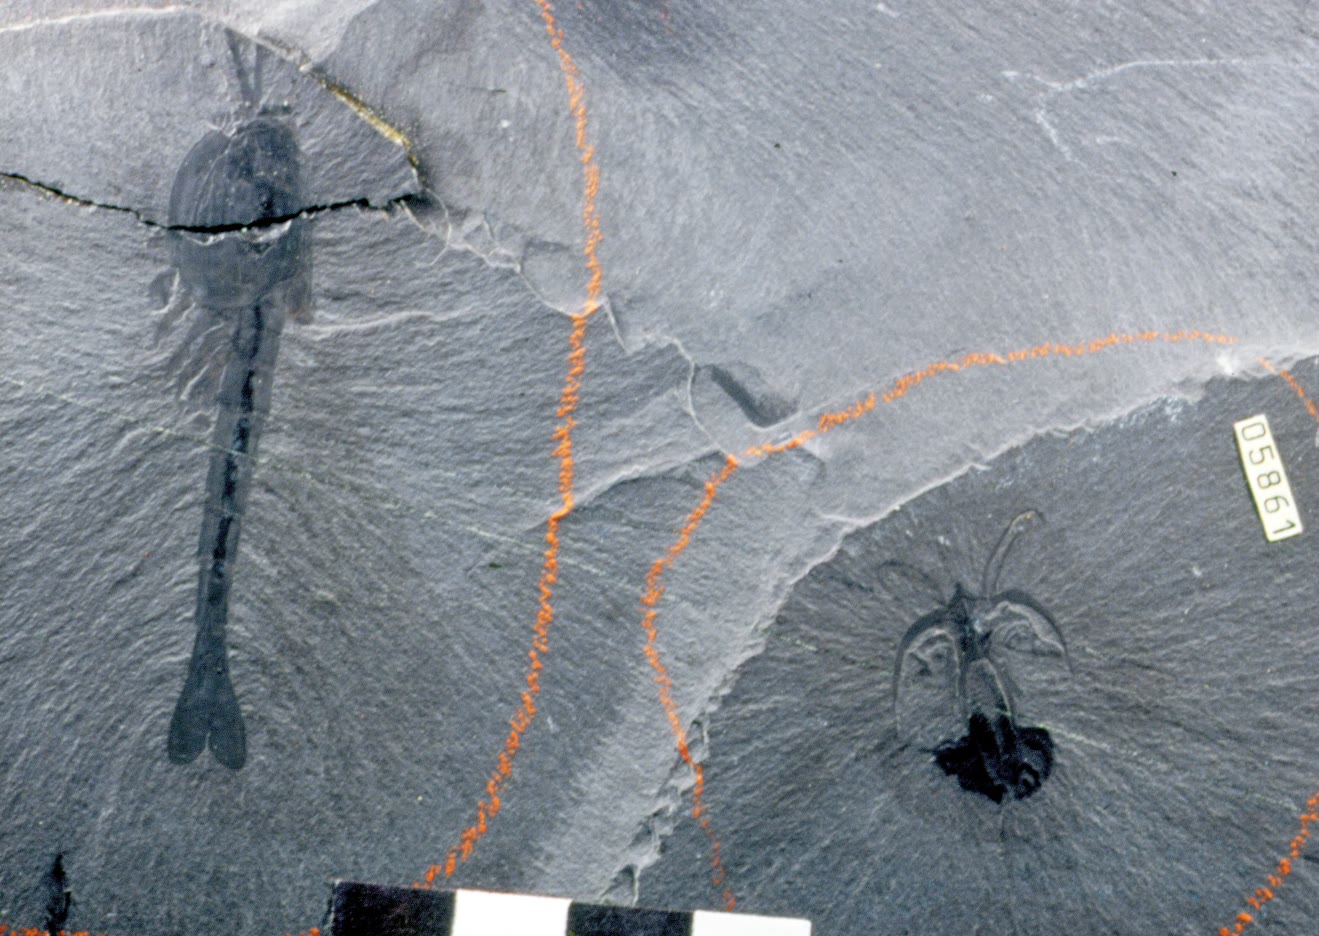
\includegraphics[width=0.72\linewidth]{images/book4/b2-20-burgess-waptia-marrella.jpg}
\par\smallskip{\small مفصليّان من طين بيرجس الصفحي، محفوظان أغشيةً داكنة من الكربون:
\emph{Waptia} (يسارًا) و\emph{Marrella} (يمينًا). الصورة: \mbox{\textdir TLT James
St.~John, CC~BY~2.0 (Wikimedia Commons)}.}
\end{omfigure}
% ledger: mussini25:burgess

\subsection*{زولنهوفن}

ترسّب الحجر الجيري الدقيق الحبيبات في زولنهوفن وآيشتيت، في بافاريا، في بحيرات شاطئية
في مطلع التيثوني، آخر أعمار الجوراسي، الذي بدأ قبل \qty{149.2}{Ma}. وهي
الموقع النموذجي لاثنتي عشرة عيّنة من \emph{Archaeopteryx}، ولكثير من الزواحف الطائرة ولأسماك
بقيت أنسجتها الرخوة بل حتى أنماط ألوانها. الحفريات هناك نادرة، لكنّ
حفظها فائق. وقد اقتُرحت عدّة ظروف، ربما عملت معًا:
مياه قاع أملح من مياه البحر بنحو ثلاث مرّات أو شديدة القلوية، تبطّئ التحلّل
البكتيري؛ وحصائر بكتيرية ختمت الجثث؛ ومياه قاع خالية من الأكسجين أبعدت
الكانسات؛ وعواصف أثارت الطين الجيري ودفنت الجثث سريعًا. وكلّ
منها يطيل زمن البقاء $1/k$ أو يقصّر زمن الدفن $h/s$.
% ledger: gerschermann21:solnhofen, rauhut18:archaeopteryx, ics4:jurassic-stages

\begin{omfigure}
\centering
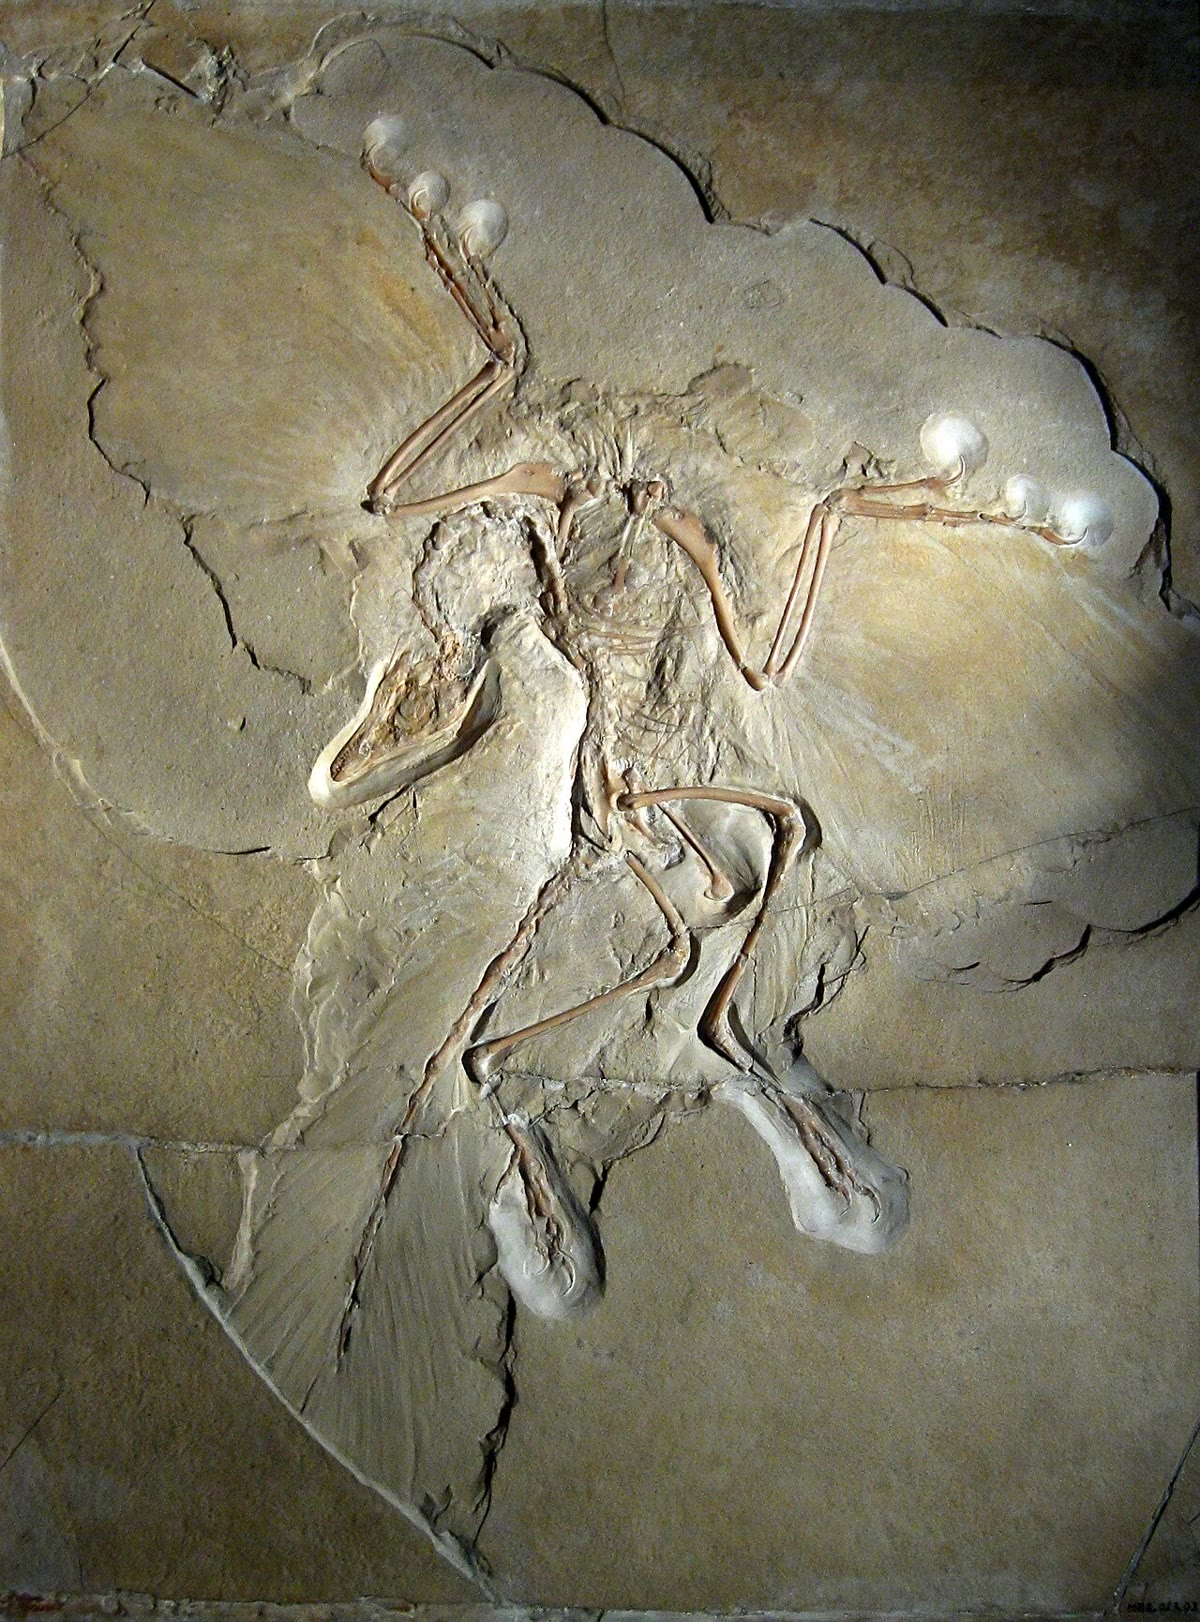
\includegraphics[width=0.5\linewidth]{images/book4/b2-20-archaeopteryx-berlin.jpg}
\par\smallskip{\small عيّنة برلين من \emph{Archaeopteryx}، من أحجار زولنهوفن
الجيرية: العظام وطبعات ريش الجناحين والذيل. الصورة: \mbox{\textdir TLT H.~Raab, CC~BY-SA~3.0
(Wikimedia Commons)}.}
\end{omfigure}
% ledger: rauhut18:archaeopteryx, gerschermann21:solnhofen

\subsection*{الحفريات ساعاتٍ}

بنى مجلد السنة الأولى الحيّز الأحيائي، وهو جسم من الطبقات تعرّفه حفرياته، والحفرية
الدليلية التي تميّزه. فما دقّة الساعة التي يصنعانها؟ قد يدوم حيّز أمونيتات جوراسي
نحو مليون سنة: فأقدم حيّزات التوارسي، المؤرَّخ بأعمار اليورانيوم--الرصاص لطبقات رماد في
الأرجنتين، يمتدّ من 183.73 إلى \qty{182.77}{Ma}. وتنقسم الحيّزات إلى آفاق، وفي الجوراسي
المتأخّر يدوم أفق الأمونيتات في المتوسط \qty{165}{kyr}. وكلّ هياكل
\emph{Archaeopteryx} تأتي من حيّز واحد يضمّ خمسة آفاق، فيُعرف الطائر على مدى
نحو 0.7 إلى مليون سنة. غير أن الحفريات لا تعطي إلا ترتيبًا؛ أمّا الأعمار بالسنين فتأتي
من طبقات الرماد المؤرَّخة باليورانيوم والرصاص، ومن الدورات الرسوبية. وتضع طبقات الرماد نفسها قاعدة التوارسي عند $183.73$، بشكّ قدره
$+0.35$ و\qty{-0.50}{Myr}، حيث يعطي الجدول الدولي \qty{184.2}{Ma}.
% ledger: alsuwaidi22:toarcian, rauhut18:archaeopteryx, ics4:jurassic-stages

\section{الحفريات شهودًا على البيئة}\label{sec:b2:palaeoenvironments:environment}

لقراءة بيئة في حفرية، يفترض الجيولوجي أن الكائن عاش حيث يعيش أقاربه
الأحياء، وأن العمليات التي تؤثّر في الرواسب اليوم أثّرت بالطريقة نفسها آنذاك.

\begin{definition}[مبدأ الحالية]\label{def:b2:palaeoenvironments:actualism}
\emph{مبدأ الحالية}\index{مبدأ الحالية} منهج تفسير السجلّات الجيولوجية الماضية بالعمليات،
وبالعلاقات بين الكائنات الحيّة وبيئتها، التي يمكن رصدها اليوم.
\end{definition}

في عام 1830 أعطى تشارلز لايل المجلد الأول من كتابه \emph{مبادئ الجيولوجيا} عنوانًا فرعيًّا هو «محاولة
لتفسير التغيّرات السابقة لسطح الأرض، بالرجوع إلى أسباب لا تزال
عاملة». وللمنهج حدود. فكثير من المجموعات منقرض، ويجب استنتاج نمط حياتها
من شكلها ومن الرواسب المحيطة بها؛ وقد لا يكون لبيئة من الماضي
نظير مطابق اليوم.
% ledger: lyell1830:title

\begin{definition}[البيئة القديمة]\label{def:b2:palaeoenvironments:palaeoenvironment}
\emph{البيئة القديمة}\index{البيئة القديمة} مجموعة الظروف الفيزيائية والكيميائية
والحيوية التي سادت حيث تكوّن صخر وحين تكوّن: الموقع، وعمق
الماء وطاقته، وملوحته وحرارته وأكسجينه، وطبيعة القاع، والحياة
عليه.
\end{definition}

\subsection*{أين عاشت الحفرية؟}

السؤال الأول هو هل عاشت الحفريات حيث ترقد.

\begin{definition}[تجمّعا الحياة والموت؛ الحفريات الأصيلة والدخيلة]\label{def:b2:palaeoenvironments:assemblages}
\emph{تجمّع الحياة}\index{تجمّع الحياة} مجموعة من حفريات كائنات عاشت
معًا، محفوظة حيث عاشت وكما عاشت؛ و\emph{تجمّع الموت}\index{تجمّع الموت}
مجموعة من بقايا جُمعت بعد الموت، وقد تخلط كائنات من أماكن مختلفة
وأزمنة مختلفة. وتكون الحفرية \emph{أصيلة}\index{الحفرية الأصيلة} إذا
حُفظت حيث عاش الكائن، و\emph{دخيلة}\index{الحفرية الدخيلة} إذا
نُقلت من مكان آخر قبل الدفن.
\end{definition}

الأدلّة هي أدلّة النقل. أصداف لا تزال مغلقة، ومرجان أو ذو مصراعين حفّار في
وضع نموّه، وأشواك دقيقة سليمة، وكلّ أعمار جماعة حاضرة: فالحفريات على
الأرجح \omterm{def:b2:palaeoenvironments:assemblages}{أصيلة}. ومصاريع مفردة مفروزة بالحجم، وشظايا بالية مكسورة، وأصداف
مركّزة عند قاعدة طبقة متدرّجة: فقد نُقلت. وتجمّع موت من الأصداف، مثل
التجمّع على القاع الساحلي المذكور أعلاه، لا يزال يحوي معظم المجتمع، لكنه يجمع سنوات كثيرة
منه في طبقة واحدة: فحفرياته متوسَّطة عبر الزمن.
% ledger: tyler25:live-dead

\subsection*{الملوحة والأكسجين}

بعض الحيوانات لا تتحمّل إلا ملوحة البحر المفتوح: وتُسمّى ضيّقة تحمّل الملوحة. فشوكيات الجلد
ورأسيات الأرجل والمرجانيات، وثلاثيات الفصوص في الباليوزوي، مجموعات نموذجية ضيّقة تحمّل الملوحة؛
ووجودها يشهد لماء بحر عادي، وغيابها عن حيوانات وفيرة قد يشهد ضدّه.
فرواسب مصبّ نهري سيلوري في فيتنام تحوي فتات نباتات، وعظام أسماك، وذوات مصراعين، وبطنيات أرجل
وقشريات صدفية، لكن لا شيء من هذه المجموعات. وتغيب شوكيات الجلد أيضًا عن أحياء تشنغجيانغ،
وهو موقع حفظ استثنائي عمره نحو 518 مليون سنة، مع أنها توجد في \omterm{def:b2:palaeoenvironments:lagerstatte}{مواقع الحفظ الاستثنائي} البحرية المفتوحة في
الكمبري: فقد عاشت حيوانات تشنغجيانغ قبالة دلتا، حيث جعل الماء العذب الملوحة تتذبذب.
% ledger: mcgairy21:stenohaline, saleh22:echinoderms, saleh22:age

ويترك الأكسجين بصمته عبر الحفّارات. فحيث يحوي ماء القاع أكسجينًا، تخلط الحيوانات
الرواسب وتدمّر تصفّحها الدقيق؛ وحيث لا يحوي شيئًا منه، تبقى الصفائح، وتغيب الجحور
ويتكوّن البيريت، كما في الأطيان الصفحية السوداء \omterm{def:b2:phanerozoic-earth:oae}{لأحداث نقص الأكسجين المحيطي} في
\cref{ch:b2:phanerozoic-earth}. وغياب الحفّارات نفسه هو ما حمى جثث طين بيرجس
الصفحي.
% ledger: mussini25:burgess

\subsection*{السحنات الأثرية}

الحفريات الأثرية أفضل الشهود على القاع، لأنها لم تُنقل. فصانعوها
يستجيبون لطاقة الماء، وصلابة القاع، والغذاء والأكسجين،
وتتكرّر الارتباطات نفسها بين الآثار عبر دهر الحياة الظاهرة.

\begin{definition}[السحنة الأثرية]\label{def:b2:palaeoenvironments:ichnofacies}
\emph{السحنة الأثرية}\index{السحنة الأثرية} ارتباط متكرّر من الحفريات الأثرية
يعكس مجموعة من الظروف البيئية؛ وتُسمّى باسم أثر مميّز لها.
\end{definition}

على امتداد مقطع بحري، من الشاطئ إلى الحوض العميق، تتعاقب أربع سحنات أثرية بحرية
(الشكل أدناه). سحنة \emph{Skolithos} الأثرية، التي تسودها جحور سكنى عمودية أسطوانية أو
على شكل الحرف U لآكلات المعلّقات، مع قليل من الآثار الأفقية، نموذجية
للشاطئ الأمامي والوجه الشاطئي. وسحنة \emph{Cruziana} الأثرية، التي تسودها جحور
آكلات الرواسب، مع آثار الراعيات واللواحم وآكلات المعلّقات، نموذجية
للمنطقة البعيدة عن الشاطئ: القاع الواقع بين قاعدة أمواج الطقس الهادئ، وهي العمق الذي تحرّك فوقه الأمواج العادية
الرواسب، وقاعدة أمواج العواصف، التي لا تبلغها إلا أمواج العواصف. وسحنة \emph{Zoophycos}
الأثرية، المسمّاة باسم جحر يعيد تقليب الرواسب في صفائح حلزونية حول محور
مركزي، نموذجية للرصيف القارّي تحت قاعدة أمواج العواصف وللمنحدر. وسحنة \emph{Nereites}
الأثرية، بجحورها المتعرّجة المنتظمة والحلزونية والشبكية، التي تُقرأ مصائدَ
وحدائقَ لحيوانات وجدت قليلًا من الغذاء، نموذجية للبحر العميق وراء حافة الرصيف. وفي
الخلجان والمصبّات قليلة الملوحة، القاعدة هي سحنة Cruziana أثرية قليلة الأنواع.
% ledger: buatois20:ichnofacies, miguez21:ichnofacies, zhang15:zoophycos, buatois25:graphoglyptids, paz23:nereites

\begin{omfigure}
\centering
\begin{tikzpicture}[font=\scriptsize, x=1cm, y=1cm]
% sea and floor (schematic, not to scale)
\fill[omSea!20] (0.6,0) -- (14,0) -- (14,-3.6) -- (11.2,-3.6) -- (9.6,-1.9) -- (6.2,-1.5)
  -- (3.2,-0.9) -- (1.2,-0.15) -- cycle;
\fill[omLithSand!45] (0,0.25) -- (0.6,0) -- (1.2,-0.15) -- (3.2,-0.9) -- (6.2,-1.5)
  -- (9.6,-1.9) -- (11.2,-3.6) -- (14,-3.6) -- (14,-4.3) -- (0,-4.3) -- cycle;
\draw[black!70, line width=0.6pt] (0,0.25) -- (0.6,0) -- (1.2,-0.15) -- (3.2,-0.9) -- (6.2,-1.5)
  -- (9.6,-1.9) -- (11.2,-3.6) -- (14,-3.6);
\draw[omSea!80!black, line width=0.6pt] (0.6,0) -- (14,0);
\node[anchor=south east, omSea!80!black] at (14,0) {مستوى البحر};
% wave bases
\draw[dashed, black!60] (2.133,-0.5) -- (14,-0.5) node[anchor=south east, black!70] {قاعدة أمواج الطقس الهادئ};
\draw[dashed, black!60] (4.7,-1.2) -- (14,-1.2) node[anchor=south east, black!70] {قاعدة أمواج العواصف};
% zone labels
\node[align=center] at (1.9,0.55) {\foreignlanguage{arabic}{الشاطئ الأمامي،}\\الوجه الشاطئي};
\node[align=center] at (4.6,0.55) {بعيدًا عن الشاطئ};
\node[align=center] at (8.0,0.55) {الرصيف};
\node[align=center] at (10.5,0.55) {المنحدر};
\node[align=center] at (12.7,0.55) {الحوض};
% Skolithos: vertical tubes
\foreach \x in {1.75,1.95,2.15,2.35} {\draw[black!80, line width=0.7pt] (\x,{-0.15-0.375*(\x-1.2)}) -- ++(0,-0.55);}
\node[align=center] at (2.1,-2.15) {\textbf{\emph{Skolithos}}\\أنابيب عمودية};
% Cruziana: horizontal bilobed trails
\foreach \x in {4.0,4.8} {\draw[black!80, line width=0.6pt] (\x,-1.45) .. controls ++(0.2,0.08) .. ++(0.5,0);
  \draw[black!80, line width=0.6pt] (\x,-1.53) .. controls ++(0.2,-0.08) .. ++(0.5,0);}
\node[align=center] at (4.7,-2.35) {\textbf{\emph{Cruziana}}\\\foreignlanguage{arabic}{جحور تغذٍّ،}\\آثار رعي};
% Zoophycos: spreite arcs
\foreach \r in {0.12,0.22,0.32} {\draw[black!80, line width=0.5pt] (8.0,-2.25) ++(-\r,0) arc (180:360:\r cm and 0.5*\r cm);}
\draw[black!80, line width=0.6pt] (8.0,-2.25) -- (8.0,-1.8);
\node[align=center] at (8.0,-3.05) {\textbf{\emph{Zoophycos}}\\صفائح\\حلزونية};
% Nereites: meander
\draw[black!80, line width=0.6pt, domain=0:2.2, samples=80, smooth] plot (12.0+\x*0.5,{-3.9+0.12*sin(\x*720)});
\node[align=center, anchor=north] at (12.5,-4.35) {\textbf{\emph{Nereites}}\\تعرّجات، شبكات};
\end{tikzpicture}
\par\smallskip{\small السحنات الأثرية البحرية الأربع في نموذج زايلاخر على امتداد مقطع من
الشاطئ إلى الحوض العميق، مع رسم لأثر مميّز لكلّ منها؛ والأعماق ليست على
مقياس الرسم. تستجيب الآثار للطاقة والغذاء والأكسجين أكثر ممّا تستجيب للعمق ذاته.}
\end{omfigure}
% ledger: buatois20:ichnofacies, miguez21:ichnofacies, zhang15:zoophycos, buatois25:graphoglyptids, paz23:nereites

العمق لا يؤثّر مباشرة. ففي قناة بحرية عميقة، حيث تيّارات العكارة قويّة، تظهر جحور
عمودية من سحنة Skolithos الأثرية تحت أيّ قاعدة أمواج بكثير؛ وقرب دلتا، حيث يتدفّق الماء
العذب والطين، تكون آثار المنطقة البعيدة عن الشاطئ أفقر منها في غيرها. وقد تنقّل الصانعون أيضًا
عبر الزمن: فالجحر \emph{Zoophycos} عاش على الرصيف في الباليوزوي، وعلى الرصيف السفلي
والمنحدر في الميزوزوي، وفي البحر العميق في السينوزوي. \omterm{def:b2:palaeoenvironments:ichnofacies}{فالسحنة الأثرية} تسجّل
الظروف على القاع، ولا يُستنتج العمق منها إلا استنتاجًا، ويجب أن يستعمل الاستنتاج
عمر الصخر.
% ledger: buatois20:ichnofacies, zhang15:zoophycos

\begin{inthefield}[عدّ الحفريات طبقةً طبقة]
عالم الحفريات الذي يعيد بناء بيئة من مقطع يسجّل كلّ طبقة بصخريّتها
وسماكتها وبناها الرسوبية، ثم بحفرياتها: أيّ المجموعات، وكم منها،
وهل الأصداف كاملة أم مكسورة، مغلقة أم مفتوحة، مفروزة أم لا، وفي أيّ وضع ترقد.
وتُسجَّل الحفريات الأثرية حيث تُرى، على أسطح التطبّق وفي الوجوه العمودية،
مع العمق الذي تبلغه الجحور. ولأن الصدفة قد تُنقل والجحر لا يُنقل، تُحفظ
القائمتان منفصلتين؛ وتُقرأ البيئة من الآثار أوّلًا، ثم تُفحص الحفريات الجسمية
بحثًا عن علامات النقل.
\end{inthefield}

\begin{omfigure}
\centering
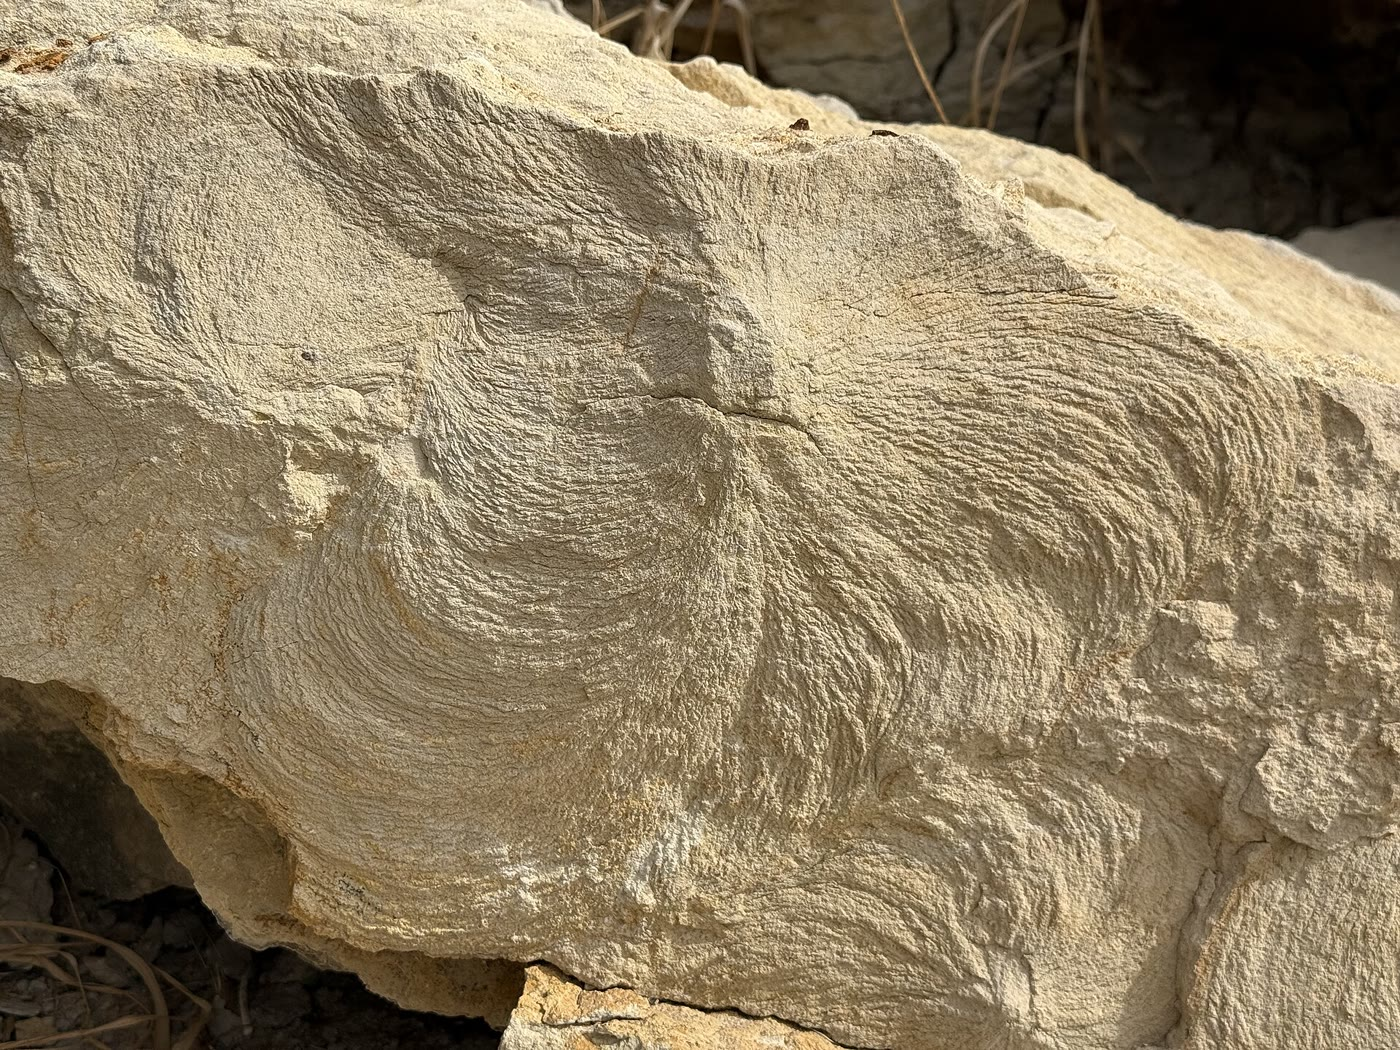
\includegraphics[width=0.5\linewidth]{images/book4/b2-20-zoophycos.jpg}
\par\smallskip{\small \emph{Zoophycos} في كتلة في ساغريش، البرتغال: الأقواس هي صفائح
صفيحة حلزونية من رواسب أُعيد تقليبها. الصورة: \mbox{\textdir TLT Amada44, CC~BY~4.0 (Wikimedia Commons)}.}
\end{omfigure}
% ledger: zhang15:zoophycos

\section{قراءة بحر زائل}\label{sec:b2:palaeoenvironments:varden}

تتجاور البيئات: شاطئ، وقاع بعيد عن الشاطئ، ورصيف أعمق. فحين يرتفع البحر أو
يهبط القاع، تتقدّم كلّ بيئة نحو اليابسة فوق جارتها، وتأتي رواسبها لترقد
فوق رواسب الجارة. فتتابعٌ رأسيّ للسحنات، بلا انقطاع، يكرّر إذن
ترتيب البيئات التي كانت متجاورة؛ ويجعل مجلد السنة الثالثة هذه القاعدة،
قانون فالتر، نقطة انطلاقه. والسجلّ المقروء من الأسفل إلى الأعلى شريط يصوّر الساحل وهو يتحرّك
عبر مكان واحد.

ويقدّم غطاء تلال فاردن، المنطقة المتخيَّلة في هذه السلسلة، مثالًا كاملًا. فسماكاته
هي سماكات نموذج المنطقة؛ والحفريات في الشكل أدناه متخيَّلة له،
لكنّ كلًّا منها مختار ليكون ممّا تحويه صخور حقيقية من ذلك النوع. ويُعطى الحجر الجيري
التوارسي، من 184.2 إلى \qty{174.7}{Ma}، والطين الصفحي من الآليني إلى الكالوفي، من
\qty{174.7}{Ma} إلى \qty{161.5}{Ma}.
% ledger: data:b4-palaeoenv, ics4:jurassic-stages

\begin{omfigure}
\centering
% figdata/bachelor-2/palaeoenv.py part log (thicknesses from figdata/shared/region.py)
\begin{tikzpicture}[x=1cm, y=0.0165cm, font=\scriptsize]
% scale
\draw[black!70] (-0.35,0) -- (-0.35,460);
\foreach \z in {0,100,...,400} {\draw[black!70] (-0.45,\z) -- (-0.35,\z) node[left=3pt] {\z};}
\node[rotate=90, anchor=south] at (-1.15,230) {\foreignlanguage{arabic}{الارتفاع فوق قاعدة الغطاء \mbox{\textdir TLT (\unit{m})}}};
% units
\fill[lith sandstone] (0,0) rectangle (2.2,120);
\fill[lith limestone] (0,120) rectangle (2.0,180);
\fill[lith limestone] (0,180) rectangle (1.6,300);
\fill[lith shale] (0,300) rectangle (1.1,400);
\fill[om lith={icsCretaceous!35}{om limestone}] (0,400) -- (1.4,400) -- (1.4,452)
  .. controls (1.0,466) and (0.6,446) .. (0.3,458) -- (0,455) -- cycle;
\draw[black!70] (0,0) rectangle (2.2,120);
\draw[black!70] (0,120) rectangle (2.0,180);
\draw[black!70] (0,180) rectangle (1.6,300);
\draw[black!70] (0,300) rectangle (1.1,400);
\draw[black!70] (0,400) -- (1.4,400) -- (1.4,452) .. controls (1.0,466) and (0.6,446) ..
  (0.3,458) -- (0,455) -- cycle;
\node[anchor=west, font=\tiny] at (1.45,460) {قمّة محتوتة};
% unit names
\node[anchor=west, align=left] at (2.6,60) {\foreignlanguage{arabic}{\textbf{الحجر الرملي}، \mbox{\textdir TLT \qty{120}{m}}}\\الترياسي};
\node[anchor=west, align=left] at (2.6,150) {\foreignlanguage{arabic}{\textbf{الحجر الجيري الأويدي}، \mbox{\textdir TLT \qty{60}{m}}}\\التوارسي};
\node[anchor=west, align=left] at (2.6,240) {\foreignlanguage{arabic}{\textbf{الحجر الجيري الدقيق}، \mbox{\textdir TLT \qty{120}{m}}}\\التوارسي};
\node[anchor=west, align=left] at (2.6,350) {\foreignlanguage{arabic}{\textbf{الطين الصفحي}، \mbox{\textdir TLT \qty{100}{m}}}\\الآليني--الكالوفي};
\node[anchor=west, align=left] at (2.6,424) {\textbf{الطباشير}\\الطباشيري};
% content
\node[anchor=west, align=left, text width=6.9cm] at (6.3,60) {حشوات قنوات متقاطعة التطبّق على قواعد
  محفورة؛ آثار جذور؛ قطع نباتية؛ لا حفريات بحرية};
\node[anchor=west, align=left, text width=6.9cm] at (6.3,150) {\foreignlanguage{arabic}{أويدات متقاطعة التطبّق؛ أنابيب عمودية
  وجحور على شكل الحرف U؛ شظايا أصداف بالية}};
\node[anchor=west, align=left, text width=6.9cm] at (6.3,240) {قطع زنابق البحر، ذراعيات الأرجل،
  البلمنيتات، الأمونيتات؛ آثار زحف وجحور تغذٍّ؛ طبقات من أصداف مكسورة ذات قواعد
  حادّة};
\node[anchor=west, align=left, text width=6.9cm] at (6.3,350) {رمادي داكن، مصفّح في مواضع؛
  بيريت؛ أمونيتات وذوات مصراعين رقيقة الأصداف؛ جحور حلزونية ذات صفائح في الطبقات الأفتح};
\node[anchor=west, align=left, text width=6.9cm] at (6.3,424) {كوكوليثات؛ قنافذ بحر، إسفنجيات؛
  عُقد صوّان؛ محفور بالجحور في كلّ مكان};
\foreach \z in {120,180,300,400} {\draw[black!25] (2.25,\z) -- (13.2,\z);}
\node[font=\scriptsize\bfseries, anchor=south west] at (2.6,462) {الوحدة والعمر};
\node[font=\scriptsize\bfseries, anchor=south west] at (6.3,462) {ما تحويه الطبقات};
\end{tikzpicture}
\par\smallskip{\small غطاء تلال فاردن سجلًّا، مع محتوى وحداته.
السماكات هي سماكات نموذج المنطقة، ما عدا الطباشير، الذي قُطعت قمّته المحتوتة هنا
(تبلغ سماكته في المقعّر \qty{766}{m}، كما في \cref{ex:b2:palaeoenvironments:shale} أدناه)؛ ويزداد عرض العمود مع حجم الحبيبات؛
والحفريات وأعمارها متخيَّلة للمنطقة.}
\end{omfigure}
% ledger: data:b4-palaeoenv, ics4:jurassic-stages

\begin{example}[قاعدة غطاء فاردن]\label{ex:b2:palaeoenvironments:base}
يحوي الحجر الرملي حشوات قنوات على قواعد محفورة، وجذورًا وقطعًا نباتية، ولا حفرية
بحرية: فقد رسّبته الأنهار على اليابسة. والحجر الجيري الأويدي فوقه فيه أويدات متقاطعة التطبّق،
تنمو وهي تتدحرج في ماء مضطرب، وأنابيب عمودية وجحور على شكل الحرف U من سحنة Skolithos
الأثرية، وشظايا أصداف بالية، كلّها \omterm{def:b2:palaeoenvironments:assemblages}{دخيلة}: إنه ضحضاح في الوجه الشاطئي،
تجتاحه الأمواج. وبين الاثنين وصل البحر: فالتماسّ يسجّل تجاوزًا بحريًّا.
وبترتيب قانون فالتر، تلا السهلَ النهريَّ الشاطئُ، ثم الضحضاح.
\end{example}
% ledger: buatois20:ichnofacies

\subsection*{ما سرعة امتلاء قاع البحر؟}

يعطي الحيّز الأحيائي مدّة، ويعطي السجلّ سماكة، ونسبتهما معدّل. لكنّ
السماكة تقلّصت منذ ترسّب الراسب: فقد اعتُصر ماء المسام
إلى الخارج، ولا تبقى محفوظة إلا الحبيبات.

\begin{proposition}[معدّل تراكم طبقة منضغطة]\label{prop:b2:palaeoenvironments:rate}
طبقة سماكتها الحالية $h$ ومساميتها المتوسطة $\varphi$، ترسّبت على مدى الزمن $\Delta t$
بالمسامية $\varphi_0$، تراكمت بالمعدّل
\[
  r = \frac{h\,(1 - \varphi)}{(1 - \varphi_0)\,\Delta t}
\]
من الراسب الطازج، وبالمعدّل $h(1-\varphi)/\Delta t$ من الحبيبات، وهو لا يتوقّف على
$\varphi_0$.
\end{proposition}

\begin{proof}
لكلّ وحدة مساحة، تحوي الطبقة حجم الحبيبات $h(1 - \varphi)$، وهو السماكة الصلبة في
مجلد السنة الأولى. والانضغاط يطرد الماء لكنه لا يضيف حبيبات ولا يزيلها، فكان للراسب
الطازج، ذي المسامية $\varphi_0$، السماكة $h_0$ مع $h_0(1 - \varphi_0) = h(1 -
\varphi)$. وقسمة $h_0$ والسماكة الصلبة على $\Delta t$ تعطي المعدّلين.
\end{proof}

وحين لا تكون المسامية مقيسة، يعطيها قانون أثي من العمق. ويبيّن الشكل أدناه
القانون لأربع صخريّات، والعامل $(1 - \varphi(z))/(1 - \varphi_0)$ الذي يجب أن تُمطّ به
طبقة رقيقة هي الآن على العمق $z$ لتعطي سماكتها عند السطح. فالطباشير والطين الصفحي
يبدآن بماء كثير ويفقدانه بسرعة: كانت طبقة رقيقة من الطين الصفحي على عمق \qty{1000}{m} أسمك
بمقدار 1.68 مرّة حين ترسّبت، وطبقة من الطباشير أسمك بمقدار 2.19 مرّة.
% ledger: pybacktrack:compaction, pybacktrack4:limestone, data:b4-palaeoenv

\begin{omfigure}
\centering
% figdata/bachelor-2/palaeoenv.py parts poro and ratio
\begin{tikzpicture}
\begin{groupplot}[group style={group size=2 by 1, horizontal sep=1.6cm},
  width=0.46\linewidth, height=6.2cm, y dir=reverse, ymin=0, ymax=3000,
  tick label style={font=\scriptsize}, label style={font=\small}, xtick pos=bottom,
  ytick pos=left, scaled y ticks=false, yticklabel style={/pgf/number format/1000 sep={\,}}]
\nextgroupplot[xmin=0, xmax=0.75, xlabel={المسامية $\varphi$}, ylabel={العمق $z$ \babelsublr{(\unit{m})}},
  legend style={at={(0.5,1.04)}, anchor=south, draw=none, font=\scriptsize, legend columns=2}]
\addplot[omThm, line width=1pt] table[x=shale, y=z_m] {figdata/out/bachelor-2-palaeoenv-poro.dat};
\addlegendentry{طين صفحي}
\addplot[omSea!80!black, line width=1pt, dashed] table[x=sandstone, y=z_m] {figdata/out/bachelor-2-palaeoenv-poro.dat};
\addlegendentry{حجر رملي}
\addplot[black, line width=1pt, dotted] table[x=chalk, y=z_m] {figdata/out/bachelor-2-palaeoenv-poro.dat};
\addlegendentry{طباشير}
\addplot[green!45!black, line width=1pt, dash dot] table[x=limestone, y=z_m] {figdata/out/bachelor-2-palaeoenv-poro.dat};
\addlegendentry{حجر جيري}
\nextgroupplot[xmin=1, xmax=3.2, xlabel={عامل الاستعادة $(1-\varphi)/(1-\varphi_0)$}]
\addplot[omThm, line width=1pt] table[x=shale, y=z_m] {figdata/out/bachelor-2-palaeoenv-ratio.dat};
\addplot[omSea!80!black, line width=1pt, dashed] table[x=sandstone, y=z_m] {figdata/out/bachelor-2-palaeoenv-ratio.dat};
\addplot[black, line width=1pt, dotted] table[x=chalk, y=z_m] {figdata/out/bachelor-2-palaeoenv-ratio.dat};
\addplot[green!45!black, line width=1pt, dash dot] table[x=limestone, y=z_m] {figdata/out/bachelor-2-palaeoenv-ratio.dat};
\end{groupplot}
\end{tikzpicture}
\par\smallskip{\small يسارًا: المسامية بدلالة العمق وفق قانون أثي، بثوابت \babelsublr{Sclater
and Christie (1980)} للطين الصفحي والحجر الرملي والطباشير، وثوابت \babelsublr{Turer and Maynard (2003)} للحجر الجيري،
كما جدولها برنامج \babelsublr{pyBacktrack}. يمينًا: العامل الذي تُستعاد به طبقة رقيقة على العمق $z$
إلى سماكتها عند السطح.}
\end{omfigure}
% ledger: pybacktrack:compaction, pybacktrack4:limestone, data:b4-palaeoenv

\begin{example}[الطين الصفحي في فاردن]\label{ex:b2:palaeoenvironments:shale}
في مقعّر تلال فاردن تبلغ سماكة الطباشير \qty{766}{m}، فيقع الطين الصفحي بين
766 و\qty{866}{m}. وبثوابت الطين الصفحي، $\varphi_0 = 0.63$ و$\lambda =
\qty{1960}{m}$، تكون السماكة الصلبة في مجلد السنة الأولى $100 - 0.63 \times 1960 \times
(e^{-766/1960} - e^{-866/1960}) = \qty{58.4}{m}$، أي مسامية متوسطة قدرها 0.416. وإذا أُعيدت الطبقة إلى
السطح بالحبيبات نفسها، صارت سماكتها \qty{148.6}{m}. وعلى مدى \qty{13.2}{Myr} من
قاعدة الآليني إلى قمّة الكالوفي، تراكم الطين الصفحي بمعدّل $100/13.2 =
\qty{7.6}{m}$ لكل مليون سنة بسماكته الحالية، و$148.6/13.2 = \qty{11.3}{m}$ لكل مليون
سنة من الطين الطازج، و\qty{4.4}{m} لكل مليون سنة من الحبيبات. فالسماكة الحالية
تبخس المعدّل بمقدار الثلث.
\end{example}
% ledger: data:b4-palaeoenv, pybacktrack:compaction, ics4:jurassic-stages

ربما رقد الطين الصفحي يومًا على عمق أكبر أيضًا، تحت طباشير حُتّ منذئذ؛ فيكون التصحيح عندئذ
حدًّا أدنى. وتطبّق مسألة نهاية الأسبوع القضية على الحجر الجيري، حيث قيست
المسامية.

\section*{التمارين}\label{sec:b2:palaeoenvironments:exercises}

معطيات التمارين، ما لم يُذكر غير ذلك: قانون أثي $\varphi = \varphi_0 e^{-z/\lambda}$
مع $\varphi_0 = 0.63$ و$\lambda = \qty{1960}{m}$ (الطين الصفحي)، و$0.49$ و\qty{3704}{m} (الحجر الرملي)،
و$0.70$ و\qty{1408}{m} (الطباشير)، و$0.51$ و\qty{4545}{m} (الحجر الجيري)؛ والكالسيت \qty{2710}{kg.m^{-3}}،
وماء المسام \qty{1000}{kg.m^{-3}}؛ وأعمار الجدول الدولي: التوارسي من 184.2 إلى
\qty{174.7}{Ma}.
% ledger: pybacktrack:compaction, pybacktrack4:limestone, ics4:jurassic-stages

\begin{exercise}[$\star$]\label{exo:b2:palaeoenvironments:1}
في 51 موقعًا من قاع ساحلي، وُجد 135 نوعًا من اللافقاريات حيًّا، و150 بين الأصداف
والهياكل الميتة على القاع، و112 لها سجلّ أحفوري أيضًا. (أ) عبّر عن العدد الثالث
كسرًا من كلّ من العددين الأوّلين. (ب) كيف يمكن أن يفوق عدد الميتة عدد الحيّة؟ (ج)
أيّ مجموعات التغذّي تتوقّع أن تكون ممثّلة تمثيلًا ناقصًا بين الميتة، ولماذا؟
\end{exercise}
% ledger: tyler25:live-dead, tyler25:soft-bodied

\begin{exercise}[$\star$]\label{exo:b2:palaeoenvironments:2}
يدوم أفق أمونيتات من الجوراسي المتأخّر في المتوسط \qty{165}{kyr}. (أ) كم تدوم خمسة آفاق؟
قارن بالمدّة من 0.7 إلى مليون سنة المعطاة للطائر \emph{Archaeopteryx}. (ب) يمتدّ أقدم حيّزات
التوارسي من 183.73 إلى \qty{182.77}{Ma}: كم أفقًا متوسّط الطول يسع؟
(ج) لماذا تهمّ الآفاقُ، لا الحيّزات، في تتبّع تطوّر سلالة؟
\end{exercise}
% ledger: rauhut18:archaeopteryx, alsuwaidi22:toarcian

\begin{exercise}[$\star$]\label{exo:b2:palaeoenvironments:3}
سمِّ \omterm{def:b2:palaeoenvironments:ichnofacies}{السحنة الأثرية} والموقع لكلّ مجموعة آثار. (أ) آثار رعي متعرّجة وشبكات جحور منتظمة
على قواعد عكرات رقيقة. (ب) أنابيب عمودية متقاربة في رمل نظيف
متقاطع التطبّق. (ج) جحور أفقية وفيرة لآكلات الرواسب وآثار رعي في طبقات
غرينية بين رمال العواصف. (د) جحور حلزونية ذات صفائح في طين دقيق داكن بلا تموّجات
أمواج، في صخور من الميزوزوي.
\end{exercise}
% ledger: buatois20:ichnofacies, paz23:nereites

\begin{exercise}[$\star$]\label{exo:b2:palaeoenvironments:4}
تحوي الطبقة A زنابق البحر وذراعيات الأرجل والمرجانيات وثلاثيات الفصوص؛ وتحوي الطبقة B، من العمر نفسه، فتات
نباتات، وعظام أسماك، وقليلًا من ذوات المصراعين وبطنيات الأرجل، وأفرادًا كثيرين من نوعين فقط من
القشريات الصدفية. (أ) ماذا تقول كلّ منهما عن ملوحة مائها؟ (ب) تفتقر الطبقة B إلى مجموعات
الطبقة A: لماذا يكون هذا الغياب حجّة، في حين أن غياب حفرية واحدة عن طبقة واحدة ليس كذلك؟
(ج) أيّ ملاحظات أخرى تختبر تفسير الطبقة B؟
\end{exercise}
% ledger: mcgairy21:stenohaline, saleh22:echinoderms

\begin{exercise}[$\star\star$]\label{exo:b2:palaeoenvironments:5}
استعمل \cref{prop:b2:palaeoenvironments:burial} مع صدفة
\cref{ex:b2:palaeoenvironments:shell}، $k = \qty{0.05}{yr^{-1}}$ و$h = \qty{0.1}{m}$. (أ)
أوجد معدّل الترسيب الذي تبلغ عنده نصف الأصداف مأمنها. (ب) بأيّ عامل يتغيّر $P$
حين يُنصَّف المعدّل من تلك القيمة؟ (ج) صدفة أسمك بمرّتين تبقى على القاع ضعف
المدّة. عند \qty{1}{mm.yr^{-1}}، كم يزيد احتمال حفظها؟ (د) ماذا
يعني هذا لنسب الأصداف الرقيقة والسميكة في تجمّع أحفوري؟
\end{exercise}
% ledger: tyler25:soft-bodied

\begin{exercise}[$\star\star$]\label{exo:b2:palaeoenvironments:6}
تؤرّخ طبقات الرماد قاعدة التوارسي في تشاكاي ميليوي عند $183.73$، $+0.35$، \qty{-0.50}{Myr}؛
ويعطي الجدول الدولي \qty{184.2}{Ma}. (أ) هل قيمة الجدول ضمن الشكّ؟
وبكم تتجاوز الحدّ الأعلى؟ (ب) ينتهي أقدم حيّزات التوارسي عند
\qty{182.77}{Ma}: أوجد مدّته. (ج) افترض أن سماكة هذا الحيّز \qty{6}{m} في مقطع:
فما معدّل التراكم؟ (د) لماذا يمكن أن يكون الحيّز الأحيائي واحدًا في الزمن في كلّ مكان مع أن
سماكته تختلف من مكان إلى آخر؟
\end{exercise}
% ledger: alsuwaidi22:toarcian, ics4:jurassic-stages

\begin{exercise}[$\star\star$]\label{exo:b2:palaeoenvironments:7}
في مقعّر فاردن يقع الحجر الرملي بين 1046 و\qty{1166}{m} تحت سطح الأرض. (أ)
أوجد مساميته وفق قانون أثي عند قمّته وعند قاعدته، ومساميته المتوسطة، مقرّبة إلى
ثلاث منازل عشرية، من متوسط القيمتين. (ب) أوجد سماكته الصلبة. (ج) أعده إلى
السطح بعامل الطبقة الرقيقة عند المسامية المتوسطة. (د) تعطي الاستعادة الدقيقة
\qty{147.0}{m}. لماذا يكون تقدير الطبقة الرقيقة أكبر قليلًا ممّا ينبغي؟
\end{exercise}
% ledger: data:b4-palaeoenv, pybacktrack:compaction

\begin{exercise}[$\star\star$]\label{exo:b2:palaeoenvironments:8}
يقرأ سجلّ الكثافة \qty{2573}{kg.m^{-3}} في حجر فاردن الجيري، المؤلَّف من حبيبات كالسيت مع
ماء في المسام. (أ) بيّن أن المسامية $\varphi = (\rho_{\text{حبيبة}} -
\rho)/(\rho_{\text{حبيبة}} - \rho_{\text{ماء}})$ واحسبها. (ب) عند منتصف عمق
الحجر الجيري في المقعّر، \qty{956}{m}، بماذا يتنبّأ قانون أثي بثوابت الحجر الجيري؟
(ج) أيّ عملية من عمليات التحوّل الرسوبي يمكن أن تفسّر الفرق؟
\end{exercise}
% ledger: pybacktrack4:limestone, data:b4-palaeoenv

\begin{exercise}[$\star\star$]\label{exo:b2:palaeoenvironments:9}
يُظهر جرف من صخور جوراسية من القاعدة إلى الأعلى: عكرات رقيقة ذات تعرّجات منتظمة وشبكات
جحور؛ وطينًا داكنًا بجحور حلزونية ذات صفائح؛ وطبقات غرينية بجحور آكلات الرواسب بين
رمال العواصف؛ ورملًا نظيفًا متقاطع التطبّق ذا
أنابيب عمودية؛ ثم فحمًا بجذور. (أ) فسّر كلّ جزء. (ب) هل تعمّق الماء أم
ضحل؟ (ج) اذكر سببين يمكن أن ينتجا هذا التتابع، وقل ما الذي يفصل
بينهما. (د) لماذا تكون القفزة الحادّة من الجزء الأول إلى الرابع، دون الأجزاء الأخرى،
إنذارًا؟
\end{exercise}
% ledger: buatois20:ichnofacies, paz23:nereites

\begin{exercise}[$\star\star\star$]\label{exo:b2:palaeoenvironments:10}
حيوان رخو الجسم يبقى على القاع سنة في المتوسط ($k = \qty{1}{yr^{-1}}$)،
وصدفة قرنًا؛ وكلاهما في مأمن تحت $h = \qty{0.1}{m}$. (أ) قارن فرص
حفظهما عند 1 و10 و\qty{100}{mm.yr^{-1}}. (ب) أوجد المعدّل الذي يُحفظ عنده جسم رخو واحد من كلّ
مئة. (ج) هل هذا المعدّل معقول على مدى أشهر متواصلة؟ وأيّ نوع من الرواسب يدفن
القاع أسرع؟ (د) أيّ فرضيات \cref{prop:b2:palaeoenvironments:burial} تسقط في مثل هذا
الراسب، وكيف تسلك الصيغة حين تسقط؟
\end{exercise}

\begin{exercise}[$\star\star\star$]\label{exo:b2:palaeoenvironments:11}
(أ) بيّن أن عامل الطبقة الرقيقة $(1 - \varphi(z))/(1 - \varphi_0)$ ينتج من
\cref{prop:b2:palaeoenvironments:rate}. (ب) طبّقه عند منتصف عمق طين فاردن الصفحي،
\qty{816}{m}، لاستعادة \qty{100}{m} من الطين الصفحي. (ج) قارن بالقيمة الدقيقة \qty{148.6}{m} في
\cref{ex:b2:palaeoenvironments:shale}، وفسّر إشارة الفرق. (د) بيّن أن
معدّل الحبيبات، بخلاف معدّل الراسب الطازج، يمكن مقارنته بين طين صفحي وحجر جيري
دون معرفة مقدار مسامية كلّ منهما حين ترسّب.
\end{exercise}
% ledger: data:b4-palaeoenv, pybacktrack:compaction

\begin{exercise}[$\star\star\star$]\label{exo:b2:palaeoenvironments:12}
افترض أن آفاق الأمونيتات في التوارسي تدوم \qty{165}{kyr} في المتوسط، مثل آفاق الجوراسي المتأخّر.
(أ) كم أفقًا يسع الحجر الجيري في فاردن، وسماكته \qty{180}{m}؟ (ب) ما سماكة
الحجر الجيري التي يمثّلها أفق واحد اليوم، وما سماكة الراسب الطازج، علمًا بأن
سماكة الطبقة كانت \qty{338}{m} حين ترسّبت؟ (ج) ليتأكّد الجيولوجي من العثور على كلّ أفق،
يأخذ عيّنات على مسافات لا تزيد على نصف تلك السماكة الحالية: فما هذه المسافة، وكم
عيّنة؟ (د) لماذا قد تغيب بعض الآفاق مع ذلك؟
\end{exercise}
% ledger: rauhut18:archaeopteryx, ics4:jurassic-stages, data:b4-palaeoenv

\begin{problem}[{مسألة نهاية الأسبوع --- بحر تلال فاردن الجوراسي}]\label{pb:b2:palaeoenvironments:1}
تقرأ هذه المسألة بيئة غطاء فاردن وتاريخه، بالسجلّ الوارد في
\cref{sec:b2:palaeoenvironments:varden} ومعطيات التمارين. يميل الغطاء
بزاوية \ang{12} على جناحي الطيّات؛ وفي المقعّر تخترقه بئر حفرًا.

\medskip\noindent\textbf{الجزء الأول --- الصخور وسماكتها.}
\begin{enumerate}
  \item على أرض مستوية على أحد الجناحين، يتكشّف الحجر الجيري على عرض \qty{866}{m}، مقيسًا
        عموديًّا على المضرب. أوجد سماكته الحقيقية.
  \item يتكشّف الطين الصفحي على \qty{481}{m}. أوجد سماكته.
  \item أيّ الوحدات أقدم، وبأيّ مبدأ؟
  \item في البئر، يبدأ الطين الصفحي عند \qty{766}{m}، والحجر الجيري عند \qty{866}{m}،
        والحجر الرملي عند \qty{1046}{m} تحت سطح الأرض. تحقّق من السماكات.
  \item يقطع سطح الأرض الطباشير. ماذا يمكن القول عن سماكته حين
        انحسر بحر الطباشيري؟
  \item أوجد مسامية الطباشير عند السطح وعند قاعدة الطباشير في البئر.
\end{enumerate}

\medskip\noindent\textbf{الجزء الثاني --- البيئات.}
\begin{enumerate}[resume]
  \item ماذا تقول زنابق البحر وذراعيات الأرجل والبلمنيتات والأمونيتات في الحجر الجيري الدقيق
        عن مائه؟
  \item أيّ سحنة أثرية تؤلّف آثاره، وفي أيّ جزء من المقطع؟
  \item ماذا تسجّل طبقاته من الأصداف المكسورة ذات القواعد الحادّة؟
  \item الطين الصفحي داكن، مصفّح في مواضع، فيه بيريت وقليل من الجحور. ماذا يقول ذلك
        عن ماء القاع؟
  \item تحوي طبقاته الأفتح جحورًا حلزونية ذات صفائح. أيّ سحنة أثرية، وأيّ موقع؟
  \item هل أمونيتات الطين الصفحي جزء من تجمّع حياة للقاع؟ علّل.
\end{enumerate}

\medskip\noindent\textbf{الجزء الثالث --- الزمن والمعدّلات.} تحوي أدنى طبقات الحجر الجيري
أمونيتات أوّل حيّز في التوارسي، وأعلاها أمونيتات آخر حيّز، ويبدأ الطين الصفحي
بأوّل حيّز في الآليني.
\begin{enumerate}[resume]
  \item كم استغرق تراكم الحجر الجيري؟
  \item بأيّ معدّل، بسماكته الحالية؟
  \item يقرأ سجلّ كثافة البئر \qty{2573}{kg.m^{-3}} في الحجر الجيري. أوجد
        مساميته.
  \item يترسّب الطين الجيري بمسامية قدرها 0.51. أوجد سماكة الراسب الطازج.
  \item أوجد معدّل الراسب الطازج.
  \item أوجد معدّل الحبيبات.
  \item قارن بالطين الصفحي في \cref{ex:b2:palaeoenvironments:shale}. ماذا يوحي تغيّر
        المعدّل عن إمداد الكربونات؟
\end{enumerate}

\medskip\noindent\textbf{الجزء الرابع --- البحر فوق فاردن.}
\begin{enumerate}[resume]
  \item اقرأ العمود من الحجر الرملي إلى الطباشير. هل تقدّم البحر أم تراجع؟
  \item على المنحنى الطويل الأمد لهاك وزملائه، كان مستوى البحر العالمي أعلى من اليوم بنحو 41 و57
        و\qty{86}{m} عند 184 و174 و\qty{162}{Ma}. بكم ارتفع في أثناء
        الحجر الجيري، وفي أثناء الطين الصفحي، وفي المجموع؟
  \item افترض أن القاع انتقل من \qty{5}{m} من الماء على الضحضاح إلى \qty{60}{m} عند قمّة
        الطين الصفحي. أوجد الاستيعاب الذي نشأ من قاعدة الحجر الجيري إلى قمّة
        الطين الصفحي، باحتساب السماكتين الطازجتين للوحدتين، ومعدّله المتوسط.
  \item أيّ حصّة منه يستطيع الارتفاع العالمي تفسيرها؟ وما الذي صنع الباقي؟
  \item خلاصة القول: بأيّ معدّل تراكم الطين الجيري لحجر فاردن الجيري حين
        ترسّب؟
\end{enumerate}
\end{problem}
% ledger: data:b4-palaeoenv, ics4:jurassic-stages, pybacktrack4:limestone, pybacktrack:compaction, data:b4-sealevel, haq87:charts, buatois20:ichnofacies, mcgairy21:stenohaline
